\chapter{TENS}

\section*{Overview}
TENS applies low-voltage electrical impulses through electrodes placed on the skin to modulate pain signals and support comfort during activity or rehabilitation. The exact approach, setting, and preparation depend on the indication, anatomy, and the patient's health.


\begin{center}
\begin{minipage}{\textwidth}\centering
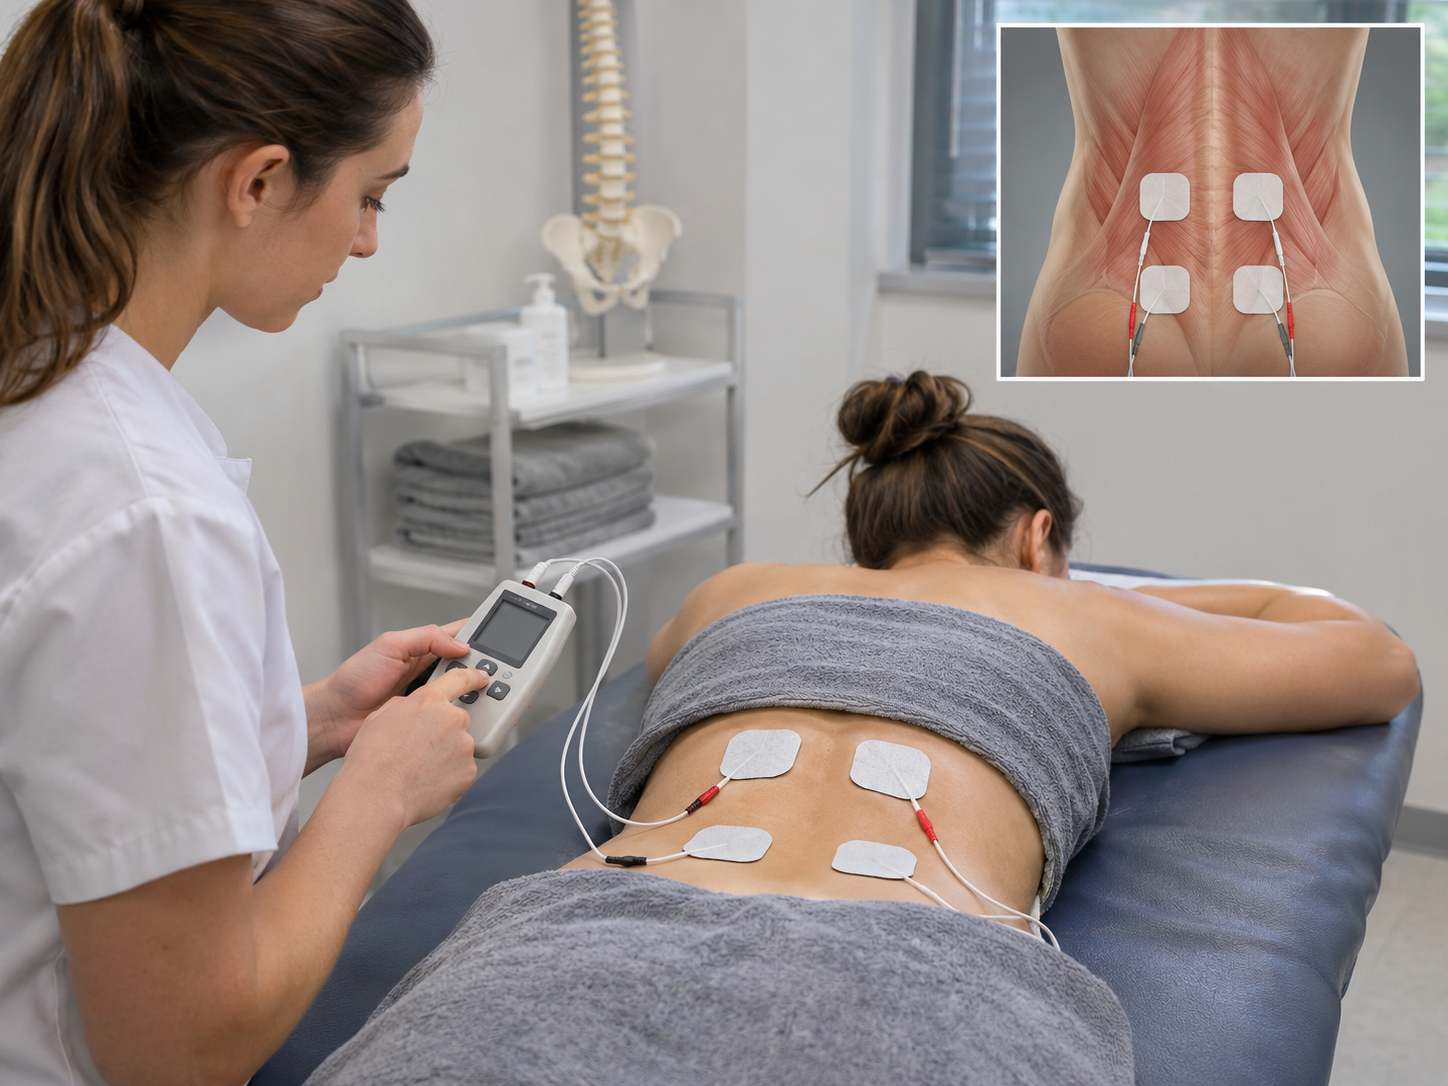
\includegraphics[width=0.82\textwidth]{images/chapters/procedure_transcutaneous_electrical_nerve_stimulation_tens_overview.png}
\captionof{figure}{TENS: Electrode pads are placed on a patient’s back and connected to a TENS unit.}
\end{minipage}
\end{center}
\section*{Common Instruments and Equipment}
The exact setup varies by technique and setting. Common items may include:
\begin{itemize}[nosep,leftmargin=*]
  \item TENS stimulator
  \item surface electrodes and connecting leads
  \item skin-preparation supplies
\end{itemize}

\section*{Why It Is Done}
It may be used as an adjunct for selected acute or chronic musculoskeletal, neuropathic, or postoperative pain. Benefit varies and it does not treat the underlying cause of pain.

\section*{How It Is Performed}
Adhesive electrodes are placed around, but not directly over, the painful area. A battery-powered device delivers adjustable pulses; intensity is increased only to a strong but comfortable sensation.

\section*{Risks and Limitations}
Skin irritation and discomfort can occur. Do not place electrodes over an implanted electronic device, the front of the neck, open wounds, or areas with absent sensation unless specifically directed by a clinician. Avoid use during bathing or driving.

\section*{Contraindications}
Electrodes should not be placed across the front of the neck, over the eyes, or across the chest without specific clinical guidance.

\section*{Precautions}
The clinician reviews implanted electrical devices, pregnancy, reduced sensation, skin infection or broken skin, and the location of electrodes.

\section*{When to Seek Medical Care}
Follow the procedure team's specific instructions. Seek urgent medical assessment for severe or worsening pain, uncontrolled bleeding, fever or signs of infection, trouble breathing, chest pain, fainting, new weakness or confusion, inability to urinate, or any rapidly worsening symptom. The appropriate warning signs depend on the procedure and the patient's medical condition.

\section*{References}
\begin{enumerate}
  \item MedlinePlus. Transcutaneous Electrical Nerve Stimulation. U.S. National Library of Medicine; 2025.
  \item Current Medical Diagnosis and Treatment. McGraw-Hill; 2025.
\end{enumerate}
\clearpage
